\documentclass{article}
\usepackage{amsmath,amssymb,amsthm,latexsym,paralist,xypic}
\input xypic % to draw the derivation tree using xymatrix
\usepackage{tikz,pgf} % to draw the FSA using tikz
\usetikzlibrary{automata}

% If you want to enlarge the page size for the text area, you can uncomment the following 
% four lines and adjust the text area as you wish by changing the values in the second { }.
%\setlength{\topmargin}{-.1in}
%\setlength{\oddsidemargin}{.2in}
%\setlength{\textwidth}{6.1in}
%\setlength{\textheight}{8.5in}

\theoremstyle{definition}
\newtheorem{problem}{Problem}
\newtheorem*{solution}{Solution}
\newtheorem*{resources}{Resources}

\newcommand{\name}[2]{\noindent\textbf{Name: #1}\hfill \textbf{Section: #2}}
\newcommand{\honor}{\noindent On my honor, as an Aggie, I have neither
  given nor received any unauthorized aid on any portion of the
  academic work included in this assignment. Furthermore, I have
  disclosed all resources (people, books, web sites, etc.) that have
  been used to prepare this homework. \\[2ex]
 \textbf{Signature:} \underline{\hspace*{10cm}} }
 
\newcommand{\checklist}{\noindent\textbf{Checklist:}
\begin{compactitem}[$\Box$] 
\item Did you type in your name and section? 
\item Did you disclose all resources that you have used? \\
(This includes all people, books, websites, etc.\ that you have consulted)
\item Did you sign that you followed the Aggie honor code? 
\item Did you solve all problems? 
\item Did you submit both the .tex and .pdf files of your homework separately 
to the correct link on eCampus?
\item Did you submit a signed hardcopy of the pdf file in class? 
\end{compactitem}
}

\newcommand{\problemset}[1]{\begin{center}\textbf{Problem Set #1}\end{center}}
\newcommand{\duedate}[2]{\begin{quote}\textbf{Due dates:} Electronic
    submission of \textsl{yourLastName-yourFirstName-hw10.tex} and 
    \textsl{yourLastName-yourFirstName-hw10.pdf} files of this homework is due on
    \textbf{#1} on \texttt{http://ecampus.tamu.edu}. You will see two separate links
    to turn in the .tex file and the .pdf file separately. Please do not archive or compress the files.  
    A signed paper copy of the pdf file is due on \textbf{#2} at the beginning of class.
    \textbf{If any of the three submissions are missing, your work will not be graded.}
    \textbf{Late submissions of any form will not be accepted.}\end{quote} }

\newcommand{\N}{\mathbf{N}}
\newcommand{\R}{\mathbf{R}}
\newcommand{\Z}{\mathbf{Z}}


\begin{document}
\vspace*{-18mm}
\begin{center}
{\large
CSCE 222 [Sections 502, 503] Discrete Structures for Computing\\[.5ex]
Spring 2017 -- Hyunyoung Lee\\}
\end{center}
\problemset{10}
\duedate{Tuesday, 5/2/2017 \textit{before} the beginning of class}{Tuesday, 5/2/2017}
\name{ Joseph Martinsen }{503}
\begin{resources} (All people, books, articles, web pages, etc.\ that
  have been consulted when producing your answers to this homework) \\
  http://madebyevan.com/fsm/
\end{resources}
\honor

\bigskip

\noindent
In this problem set, you will earn total $100+5$ (extra credit) points.

\begin{problem} (10 points)
Section 13.1, Exercise 4, page 856
\end{problem}
\begin{solution} \ \\
  \begin{enumerate}
    \item 
      \begin{align*}
        S &\rightarrow 1S \\
        &\rightarrow 11S \\
        &\rightarrow 11100S \\
        &\rightarrow 111000
      \end{align*}
      
      \item
      111001 does not belong in the language because the only production that
      terminates with a terminal is $S \rightarrow 0$ which results in every member
      in the language must end with 0, which 111001 does not.
      
      \item
      $$L(G) = \{ 1^n 0^m \vert n\ge 0, m \ge 3 \} $$
  \end{enumerate}
\end{solution}

\begin{problem} (10 points)
Section 13.1, Exercise 6 a), b), c), and d), page 856
\end{problem}
\begin{solution} \ \\
a) \\
$$L(G) = \{ abbb \}$$
b) \\
$$L(G) = \{aba, aa \} $$
c) \\
$$L(G) = \{abb, abab \} $$
d) \\
$$L(G) = \{a^{2n} \vert n \ge 2 \} \cup \{b^n \vert n \ge 1 \} $$
\end{solution}

\begin{problem} (16 points)
Section 13.1, Exercise 14, page 856
\end{problem}
\begin{solution} \ \\
  \begin{enumerate}
    \item
    \begin{align*}
      G &= (V,T,S,P) \\
      V &= \{0,1,S\} \\
      T &= \{0,1\} \\
      P &= \{S \rightarrow 10, S \rightarrow 01, S \rightarrow 101\}
    \end{align*}
    \item
    \begin{align*}
      G &= (V,T,S,P) \\
      V &= \{0,1,A,S\} \\
      T &= \{0,1\} \\
      P &= \{S \rightarrow 00A1, A \rightarrow AA, A \rightarrow 0, A \rightarrow 1 \}
    \end{align*}
    \item
    \begin{align*}
      G &= (V,T,S,P) \\
      V &= \{0,1,A,B,S\} \\
      T &= \{0,1\} \\
      P &= \{S \rightarrow A0, B \rightarrow \lambda, A \rightarrow 11B, A \rightarrow 1B1, A \rightarrow B11, B \rightarrow 0B \}^*
    \end{align*}
    *0 is not even because you can not divide up 0 objects into two groups
    \item
    \begin{align*}
      G &= (V,T,S,P) \\
      V &= \{0,1,A,B,S\} \\
      T &= \{0,1\} \\
      P &= \{S \rightarrow AB, A \rightarrow B0, B \rightarrow A1, A \rightarrow \lambda, B \rightarrow \lambda\}
    \end{align*}
  \end{enumerate}
\end{solution}

\begin{problem} (12 points)
Section 13.1, Exercise 18, page 856
\end{problem}
\begin{solution} \ \\
\begin{enumerate}
    \item
    \begin{align*}
      G &= (V,T,S,P) \\
      V &= \{0,1,A,S\} \\
      T &= \{0,1\} \\
      P &= \{S \rightarrow 0A, A \rightarrow 11A, A \rightarrow \lambda \}
    \end{align*}

    \item
    \begin{align*}
      G &= (V,T,S,P) \\
      V &= \{0,1,S\} \\
      T &= \{0,1\} \\
      P &= \{S \rightarrow 0S11, S \rightarrow \lambda \}
    \end{align*}
    \item
    \begin{align*}
      G &= (V,T,S,P) \\
      V &= \{0,1,A,S\} \\
      T &= \{0,1\} \\
      P &= \{S \rightarrow 0S0, S \rightarrow A, S \rightarrow \lambda, A \rightarrow \lambda, A \rightarrow 1A\}
    \end{align*}

\end{enumerate}
\end{solution}

\begin{problem} (10 points)
Section 13.1, Exercise 24, page 857
\end{problem}
\begin{solution} \ \\
\begin{enumerate}
  \item
  $$
  \xymatrix{
    & & S \ar[dll] \ar[dl] \ar[d] \\
    b & c & S \ar[dll] \ar[dl] \ar[d] \\
    b & b & S  \ar[d] \\
    &  & a
  }
  $$
  Results in $bcbba$
  
  \item
  $$
  \xymatrix{
    & & S \ar[dll] \ar[dl] \ar[d] \\
    b & b & S \ar[dll] \ar[dl] \ar[d] \\
    b & c & S \ar[dll] \ar[dl] \ar[d] \\
    b & b & S \ar[d] \\
    & & a
  }
  $$
  Results in $bbbcbba$
  
  \item
  $$
  \xymatrix{
    & & S \ar[dll] \ar[dl] \ar[d] \\
    b & c & S \ar[dll] \ar[dl] \ar[d] \\
    a & b & S \ar[dll] \ar[dl] \ar[d] \\
    b & b & S \ar[dll] \ar[dl] \ar[d] \\
    b & b & S \ar[dl] \ar[d] \\
    & c & b
  }
  $$
  Results in $bcabbbbbcb$
\end{enumerate}
\end{solution}

\begin{problem} (6 points)
Section 13.2, Exercise 2 a), page 864
\end{problem}
\begin{solution} 
$$
\begin{tabular}{c|cc|cc|} % the table has five columns
% f is over 2nd and 3rd columns and g over the 4th and 5th columns
& \multicolumn{2}{c|}{f} & \multicolumn{2}{c|}{g} \\
\cline{2-5} % put a line over the columns from the 2nd to the 5th
& \multicolumn{2}{c|}{Input} & \multicolumn{2}{c|}{Input} \\
State & 0 & 1 & 0 & 1 \\
\hline
$s_0$ & $s_1$ & $s_2$ & 1 & 0 \\
$s_1$ & $s_0$ & $s_3$ & 1 & 0 \\
$s_2$ & $s_3$ & $s_0$ & 0 & 0 \\
$s_3$ & $s_1$ & $s_2$ & 1 & 1 \\
\end{tabular}
$$
\end{solution}

\begin{problem} (6 points)
Section 13.2, Exercise 4, page 864
\end{problem}
\begin{solution} \ \\
 \begin{enumerate}
   \item \ \\
   \begin{table}[h]
   \begin{center}
     \begin{tabular}{c|ccccc}
       Input & 1 & 0 & 0 & 0 & 1 \\
       \hline \\
       State & $s_0$ & $s_2$ & $s_3$ & $s_1$ & $s_0$ \\
       \hline \\
       Output & 0 & 0 & 1 & 1 & 0
     \end{tabular}
   \end{center}
   Output: 00110
 \end{table}
 
   \item \ \\
   \begin{table}[h]
   \begin{center}
     \begin{tabular}{c|ccccc}
       Input & 1 & 0 & 0 & 0 & 1\\
       \hline \\
       State & $s_0$ & $s_2$ & $s_2$ & $s_2$ & $s_2$ \\
       \hline \\
       Output & 1 & 1 & 1 & 1 & 0
     \end{tabular}
   \end{center}
   Output: 11110
 \end{table}
 
   \item \ \\
   \begin{table}[h]
   \begin{center}
     \begin{tabular}{c|ccccc}
       Input & 1 & 0 & 0 & 0 & 1 \\
       \hline \\
       State & $s_0$ & $s_1$ & $s_0$ & $s_3$ & $s_1$ \\
       \hline \\
       Output & 1 & 0 & 0 & 0 & 1
     \end{tabular}
   \end{center}
   Output: 10001
 \end{table}
 
 \end{enumerate}
\end{solution}

\begin{problem} (12 points)
Section 13.3, Exercise 8, page 875
\end{problem}
\begin{solution} \ \\
\begin{enumerate}
  \item Let $ A = \{ a \} $. This results in $A^2 = \{ aa \}$. $\{ a \} \nsubseteq \{ aa \} $ which disproves the statement.
  
  \item 
  
  \item $A\{\lambda \}$ concatenated results in simply $A$ because $\lambda$ is the empty set.
  This results in $A\{\lambda \} = A$ which is the given statement.
  
  \item 
  
  \item $A^*$ contains $A^0$. $A^* A \rightarrow A^0 A = A^{0+1} = A^1 = A \neq A^0 \leftarrow A^*$. Therefore the given statement is false.  
  
  \item
  Let $A = \{\lambda, 1 \}$ which results in $A^2 = \{\lambda, 1, 11 \}$. $\vert A^2 \vert = 3$ and $\vert A \vert = 2$ which results $\vert A \vert ^2 = 4$ which is not 3 resulting in the given stament being false.
\end{enumerate}
\end{solution}

\begin{problem} (12 points)
Section 13.3, Exercise 10, page 875
\end{problem}
\begin{solution} \ \\
\begin{enumerate}
  \item Yes
  \item No
  \item Yes
  \item Yes
  \item No
  \item No
\end{enumerate}
\end{solution}

\begin{problem} (5 points)
Section 13.3, Exercise 16, page 876
\end{problem}
\begin{solution} 
$$\{\lambda \} \cup \{1\}\{0,1\}^* \cup \{0\}\{1\}^*\{0\}\{0,1\}^*$$
\end{solution}

\begin{problem} (6 points)
Section 13.3, Exercise 28, page 876
\end{problem}
\begin{solution} \ \\
% Used to draw: http://madebyevan.com/fsm/
\begin{center}
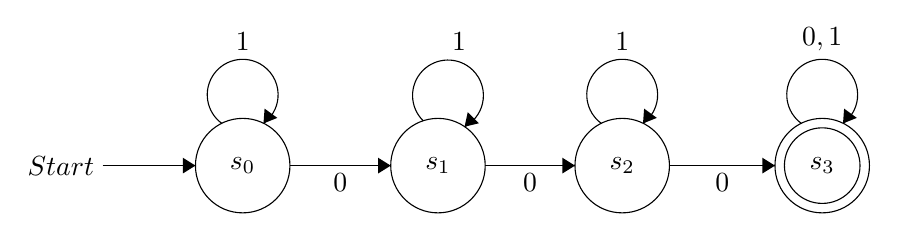
\begin{tikzpicture}[scale=0.2]
\tikzstyle{every node}+=[inner sep=0pt]
\draw [black] (10.9,-25.7) circle (3);
\draw (10.9,-25.7) node {$s_0$};
\draw [black] (23.3,-25.7) circle (3);
\draw (23.3,-25.7) node {$s_1$};
\draw [black] (35,-25.7) circle (3);
\draw (35,-25.7) node {$s_2$};
\draw [black] (47.7,-25.7) circle (3);
\draw (47.7,-25.7) node {$s_3$};
\draw [black] (47.7,-25.7) circle (2.4);
\draw [black] (13.9,-25.7) -- (20.3,-25.7);
\fill [black] (20.3,-25.7) -- (19.5,-25.2) -- (19.5,-26.2);
\draw (17.1,-26.2) node [below] {$0$};
\draw [black] (26.3,-25.7) -- (32,-25.7);
\fill [black] (32,-25.7) -- (31.2,-25.2) -- (31.2,-26.2);
\draw (29.15,-26.2) node [below] {$0$};
\draw [black] (38,-25.7) -- (44.7,-25.7);
\fill [black] (44.7,-25.7) -- (43.9,-25.2) -- (43.9,-26.2);
\draw (41.35,-26.2) node [below] {$0$};
\draw [black] (46.377,-23.02) arc (234:-54:2.25);
\draw (47.7,-18.45) node [above] {$0,1$};
\fill [black] (49.02,-23.02) -- (49.9,-22.67) -- (49.09,-22.08);
\draw [black] (33.677,-23.02) arc (234:-54:2.25);
\draw (35,-18.45) node [above] {$1$};
\fill [black] (36.32,-23.02) -- (37.2,-22.67) -- (36.39,-22.08);
\draw [black] (22.37,-22.86) arc (225.8699:-62.1301:2.25);
\draw (24.64,-18.41) node [above] {$1$};
\fill [black] (24.99,-23.23) -- (25.9,-23.01) -- (25.19,-22.31);
\draw [black] (9.577,-23.02) arc (234:-54:2.25);
\draw (10.9,-18.45) node [above] {$1$};
\fill [black] (12.22,-23.02) -- (13.1,-22.67) -- (12.29,-22.08);
\draw [black] (2,-25.7) -- (7.9,-25.7);
\draw (1.5,-25.7) node [left] {$Start$};
\fill [black] (7.9,-25.7) -- (7.1,-25.2) -- (7.1,-26.2);
\end{tikzpicture}
\end{center}

\end{solution}

\goodbreak
\checklist
\end{document}
